\documentclass{beamer}
\usepackage{graphicx,amsmath,amsfonts,amssymb,listings,tikz}
\usepackage{multimedia}
\usetheme{Montpellier}
\usecolortheme{beaver}
\beamerdefaultoverlayspecification{<+->}

% user commands
\newcommand{\weeknum}{10}

\begin{document}

\section{Group Meeting}
\title{Group Meeting \\ Week \weeknum, Spring 2019}
\author{Brandon Gusto} %
\institute{Dept. of Scientific Computing \\ Florida State University}
\date{\today}
\frame{\titlepage}

\begin{frame}{Recent Progress to Proteus}
  Following items have been added to my wavelet code over last two weeks:
  \begin{itemize}
    \item<2-> added all parameters to \texttt{flash.par}
    \item<3-> new \texttt{Matlab} script to run convergence studies, modfying \texttt{flash.par}
    \item<4-> can specify periodic domain (or not) needed for buffer region and interpolation
  \end{itemize}
\end{frame}

\begin{frame}{Convergence}
  With 1 buffer cell per side of a significant cell:
  \begin{figure}
    \center
    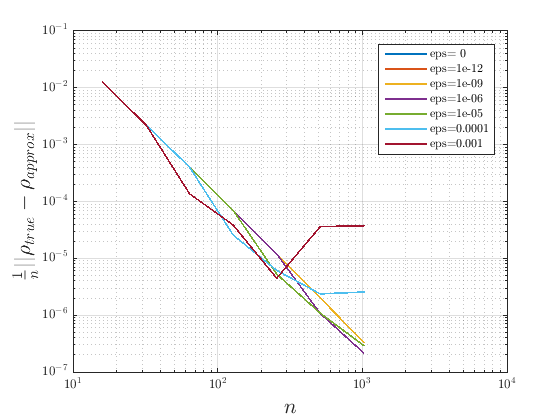
\includegraphics[scale=0.5]{buffer1.png}
  \end{figure}
\end{frame}

\begin{frame}{Convergence}
  With 2 buffer cell per side of a significant cell:
  \begin{figure}
    \center
    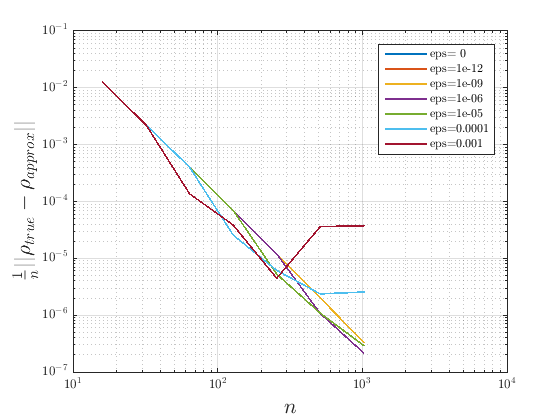
\includegraphics[scale=0.5]{buffer2.png}
  \end{figure}
\end{frame}

\begin{frame}{Convergence}
  With 3 buffer cell per side of a significant cell:
  \begin{figure}
    \center
    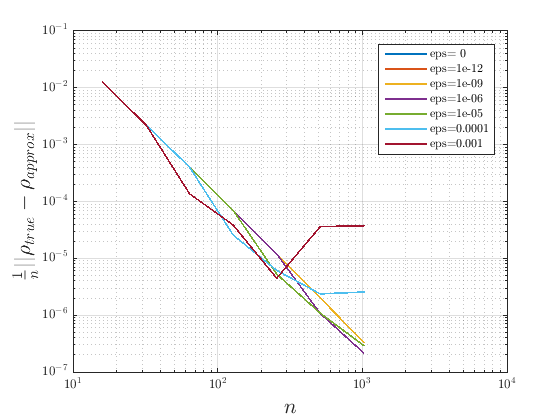
\includegraphics[scale=0.5]{buffer3.png}
  \end{figure}
\end{frame}

\begin{frame}{Convergence}
  With 4 buffer cell per side of a significant cell:
  \begin{figure}
    \center
    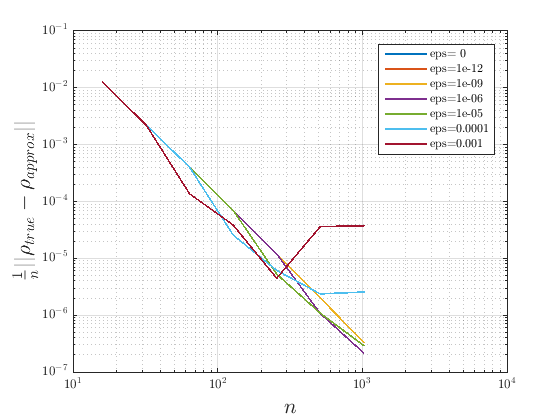
\includegraphics[scale=0.5]{buffer4.png}
  \end{figure}
\end{frame}

\end{document}
